\section{Optimointimenetelmät}

Konekoodiksi kääntäminen tuo ongelmaksi hitaan käännösvaiheen. Tämän takia modernit virtuaalikoneet sisältävät useamman kuin yhden kerroksen JIT-kääntäjiä eritasoisilla optimoinneilla. Tässä luvussa esitellään muutamia keinoja, joilla JavaScript-virtuaalikoneet ovat parantaneet tuottamansa konekoodin suorituskykyä.

\subsection{Piiloluokat}

JavaScriptin oliot käyttävät prototyyppiperintää. Tämä tarkoittaa, että oliolla voi olla toinen olio prototyyppinään, jolla on toinen olio prototyyppinään ja niin edelleen. Kun oliolta pyydetään jonkin \textit{ominaisuuden} (property) arvoa, etsitään sitä ensin itse oliosta. Jos sitä ei löydy, käydään olion prototyyppiketjua läpi, kunnes ominaisuus löytyy tai kaikki prototyypit on käyty läpi, jolloin arvo on ''undefined``. Tämä tarkoittaa, että ominaisuuksien arvot saattavat olla muistissa kaukana toisistaan ja niiden löytämiseen tarvitaan hidasta assosiatiivista hakurakennetta.

V8 esitteli ominaisuuden nimeltään \textit{piiloluokka} (hidden class)~\cite{v8design}. Piiloluokat ovat staattisia eli \textit{muuttumattomia} (immutable) luokkia, joita virtuaalikone käyttää dynaamisten JavaScript-olioiden rakenteen kuvaamiseen. Piiloluokka on tavallaan siis olion tyyppi, vaikka JavaScriptissä muuttujilla ei ole tyyppejä. Olioita voi käyttää hyvin dynaamisesti, mutta virtuaalikone olettaa, että useimmissa tapauksissa niitä käytetään melko staattisesti. Käyttämällä piiloluokkaa ikään kuin olion tyyppinä virtuaalikoneet voivat hyödyntää tehokkaita kääntämistekniikoita, joita käytetään staattisesti tyypitetyissä kielissä.

Tämä onnistuu siten, että kun olio luodaan, luodaan sille piiloluokka. Aina kun oliota muutetaan lisäämällä siihen ominaisuus, luodaan sitä vastaamaan uusi piiloluokka. Luokkaa ei voi tehdä etukäteen, koska dynaamisuuden takia on vaikea tietää ennalta millainen olio tulee rakenteeltaan olemaan.

Kuvassa~\ref{fig:hiddenclass} näkyy esimerkki Piste-nimisen olion ja sen piiloluokan muodostus. Kun konstruktorifunktiota kutsutaan, luodaan tyhjä olio, jota virtuaalikone kuvaa tyhjällä piiloluokalla \textbf{C0}. Luokkaa C0 käytetään kuvaamaan kaikkia tyhjiä olioita, joilla on sama prototyyppi. Konstruktorissa olioon liitetään ominaisuus x, jolloin virtuaalikone luo uuden piiloluokan \textbf{C1} ja lopulta y:n lisäyksen jälkeen \textbf{C2}:n. Piiloluokkiin tallennetaan tieto mihin luokkaan pitää siirtyä tietyn ominaisuuden lisäämisen jälkeen.

\begin{figure}[ht]
    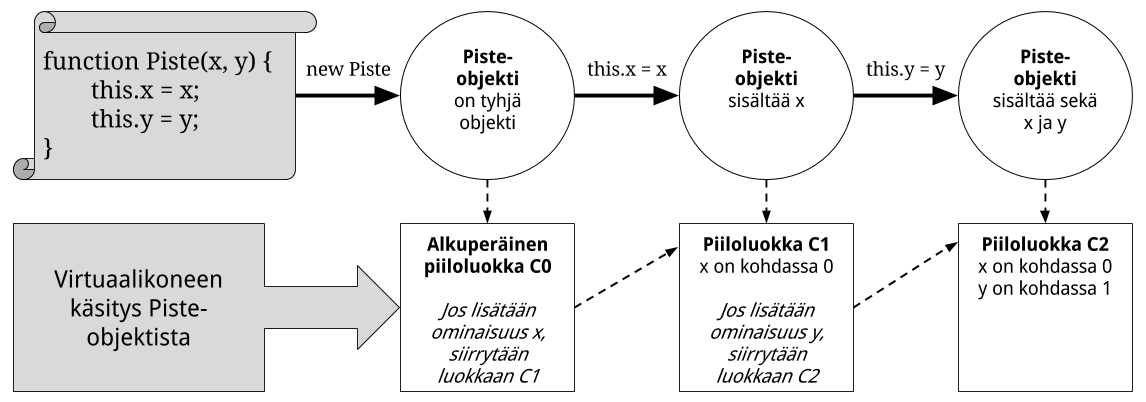
\includegraphics[width=\textwidth]{hidden-classes}
    \caption{Esimerkki piiloluokkien toimintaperiaatteesta.}
     \centering
     \label{fig:hiddenclass}
\end{figure}

Piiloluokkia ei tarvitse luoda uudestaan joka kerta kun halutaan luoda uusi Piste-olio. Riittää, että seurataan niihin sisällytettyjä tietoja siirtymistä. Kun uusi Piste-olio luodaan, päädytään lopulta samaan piiloluokkaan \textbf{C2}. Kaikki Piste-oliot ovat siis tavallaan samantyyppisiä.

Kun Piste-oliolta pyydetään esimerkiksi ominaisuuden x arvoa, virtuaalikone tietää, että olio on luokan \textbf{C2} ''tyyppinen`` ja arvo löytyy yhdellä konekäskyllä muistipaikasta 0 ilman, että täytyy tehdä hidasta hakua assosiatiivisesta hakurakenteesta. Virtuaalikone voi siis generoida tehokkaampaa konekoodia ja muistiviittaukset nopeutuvat huomattavasti.

Jos oliota muokataan uudestaan luomisen jälkeen, luodaan sille uusi piiloluokka ja optimoinnit täytyy suorittaa tälle uudelle tyypille uudestaan. Jos kaikkia ominaisuuksia ei alusteta aina samassa järjestyksessä tai niitä alustetaan ehdollisesti, se tuottaa ongelmia piiloluokkien toiminnan kannalta. Ongelmaksi muodostuu myös se, että piiloluokkaan sisällytetään koko prototyyppiketju~\cite[s.~499]{Ahn2014}, jolloin muutokset johonkin prototyyppiketjussa ylempänä olevaan objektiin pakottavat uuden piiloluokan luomisen.

\subsection{Sisällytetty välimuisti}

Yleinen olettamus on, että samalla \textit{hakupaikalla} (access site) oliot ovat usein samantyyppisiä. Tämän takia on alettu käyttämään \textit{sisällytettyä välimuistia} (inline cache)~\cite[s.~498]{Ahn2014}. Nimi tulee siitä, että välimuisti tulee osaksi generoitua konekoodia.

Esimerkiksi Piste-oliolla voi olla metodi getX, joka palauttaa x:n arvon. Keräämällä tietoa suoritusaikana virtuaalikone voi päätellä, että tässä kohtaa olio on usein Piste-olio. Virtuaalikone muokkaa konekoodia ja lisää tarkistuksen "onko olion piiloluokka sama kuin Piste-olion?". Jos oliolla on sama piiloluokka, x:n arvon lukemiseksi riittää katsoa piiloluokasta sen \textit{siirtymä} (offset) muistissa ja suorittaa yksi muistioperaatio.

V8:ssa on kolmen tyyppisiä sisällytettyjä välimuisteja: \textit{lataukselle} (load), \textit{talletukselle} (store) ja \textit{kutsumiselle} (call). Lataaminen tarkoittaa olion ominaisuuden hakemista ja talletus sen päivittämistä. Kutsuminen tarkoittaa olion metodin kutsumista ja se on samankaltainen lataamisen kanssa, sillä ensin pitää ladata metodi, joka on JavaScriptissä viittaus funktio-olioon.

Jos välimuistista tulee huti, V8 lisää uuden olion piiloluokan tarkistuksen sisällytettyyn välimuistiin. Ylimääräiset tarkistukset tekevät koodista hitaampaa, mutta tutkimusten mukaan~\cite[s.~498]{Ahn2014} suoritus välimuistin avulla voi olla parhaimmillaan monta suuruusluokkaa nopeampi kuin ilman välimuistia, joten tässä tapauksessa vaihtokauppa on kannattava.

\subsection{Roskienkeräys}

\textit{Roskienkeräys} (garbage collection) on perinteisesti toiminut melko yksinkertaisella algoritmilla nimeltään \textit{merkitse ja pyyhkäise} (mark-and-sweep). Se aloittaa merkitsemisvaiheella ja lähtee liikkeelle niin sanotusta juurisetistä olioita. Algoritmi seuraa muistiviitteitä merkiten vastaan tulleet oliot kunnes kaikki on käyty läpi. Sen jälkeen tulee pyyhkäisyvaihe. Algoritmi käy läpi koko muistin ja vapauttaa kaikki oliot, jotka eivät ole merkittyjä. Samalla algoritmi poistaa merkit seuraavaa kierrosta varten.

Ohjelman suoritus ei voi jatkua roskienkeräyksen aikana ja koko muistialueen merkitseminen ja läpikäyminen on hidasta. Tämä on suuri ongelma varsinkin animaatioiden ja interaktiivisten sovellusten tapauksessa, sillä pitkä roskienkeräystauko haittaa käytettävyyttä ja saa sovelluksen tuntumaan hitaalta vaikka muu suoritus olisikin todella nopeaa.

Ongelman ratkaisemiseksi on kehitetty erilaisia heuristiikkoja ja optimointeja. Esimerkiksi \textit{sukupolvittainen roskienkeräys} (generational garbage collection)~\cite{v8design} perustuu oletukseen, että suurin osa luoduista muistivarauksista on lyhytaikaisia. Jakamalla muistialue kahteen erikokoiseen sukupolveen, nuoreen ja vanhaan, voidaan allokoida uudet oliot pienemmälle nuorelle alueelle. Nuoren alueen voi pienempänä käsitellä nopeammin ja useammin. Jos olio selviää nuorella alueella roskienkeräyksestä, se on todennäköisesti pitkäikäisempi olio ja se siirretään vanhalle alueelle, jota käsitellään harvemmin.

%\subsection{Staattinen kertasijoitusmuoto}

%(Static single assignment form, SSA)

%https://blog.chromium.org/2010/12/new-crankshaft-for-v8.html
%An optimizing compiler which recompiles and optimizes hot code identified by the runtime profiler. It uses static single assignment form to perform optimizations such as loop-invariant code motion, linear-scan register allocation and inlining. The optimization decisions are based on type information collected while running the code produced by the base compiler.